\documentclass[letterpaper,11pt]{article}

\usepackage{geometry}
\usepackage{pslatex}
\usepackage{fancyhdr}
\usepackage{graphicx}
\usepackage{setspace}
\usepackage{amsmath, amssymb}
\usepackage{hyperref}
\geometry{ margin = 1.0in }

\pagestyle{fancy}
\lhead{{\bf CMPSC 431W}}
\chead{{\bf Database Management System}}
\rhead{{\bf \today}}

\setlength\parindent{0em}
\setlength\parskip{8pt}

\newcommand{\Paragraph}[1]{~\vspace*{-0.7\baselineskip}\\{\bf #1}}



\begin{document}

\begin{center}
	{\LARGE \bf Assignment 4 Solution}
	
	{\large
	Name: Yanjun Chen, PSU ID: yfc5289}
\end{center}

\section*{Part I: Problem 1}
\Paragraph{1. }
\begin{figure}[h]
    \centering
    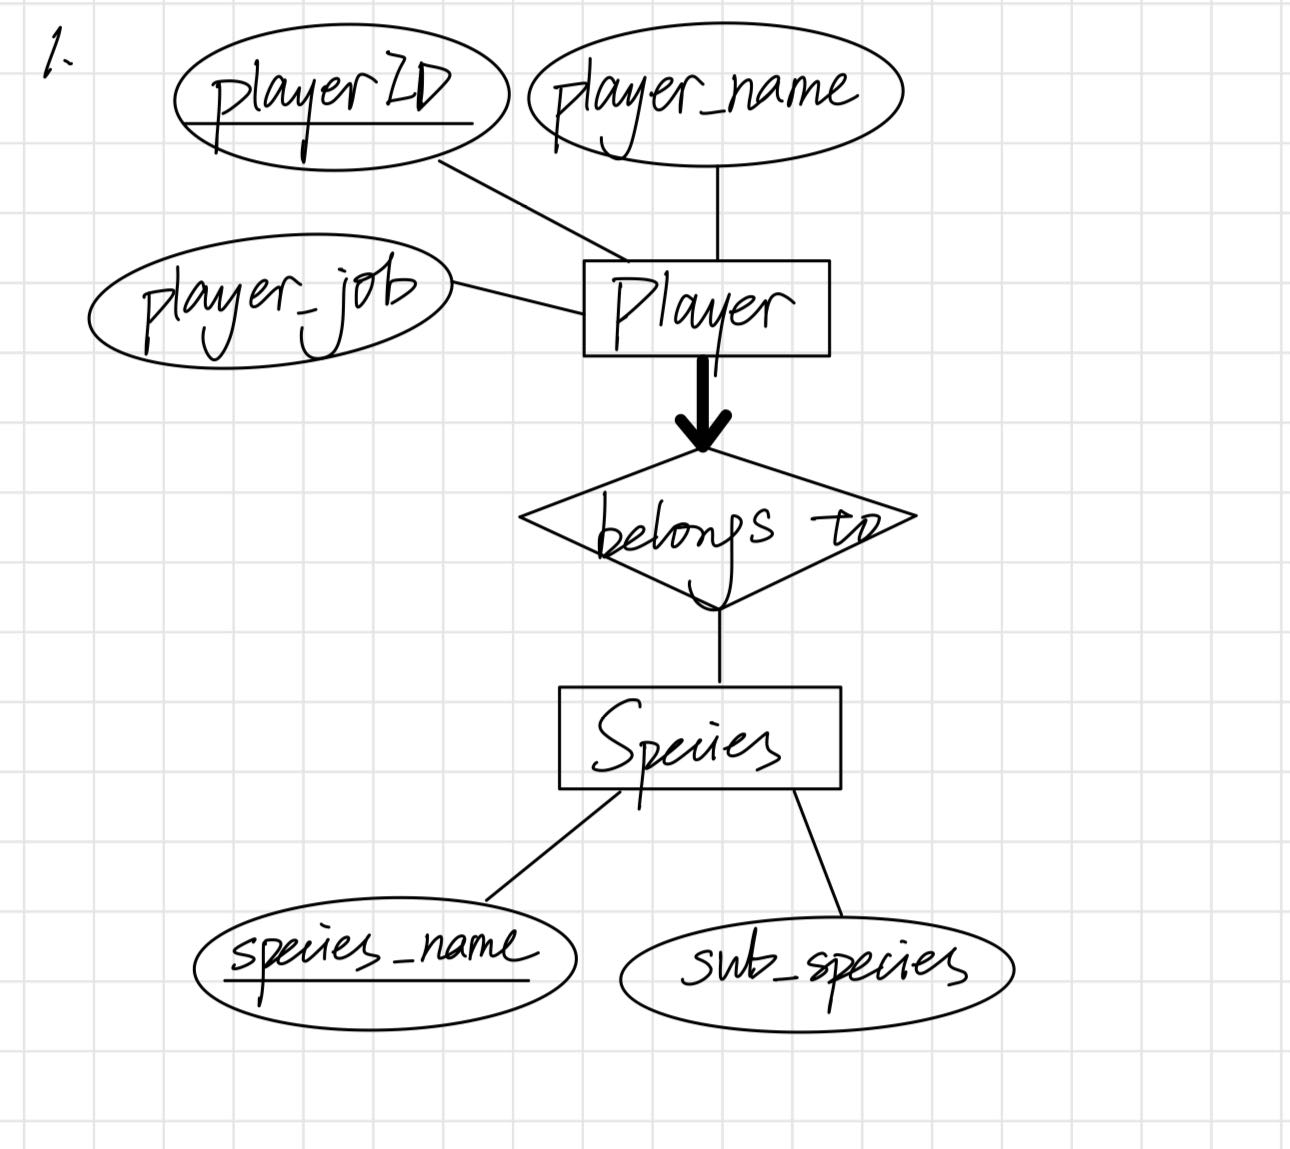
\includegraphics[width=0.5\textwidth]{p1-1-1.jpg}
\end{figure}

\Paragraph{2.}
\begin{figure}[h]
    \centering
    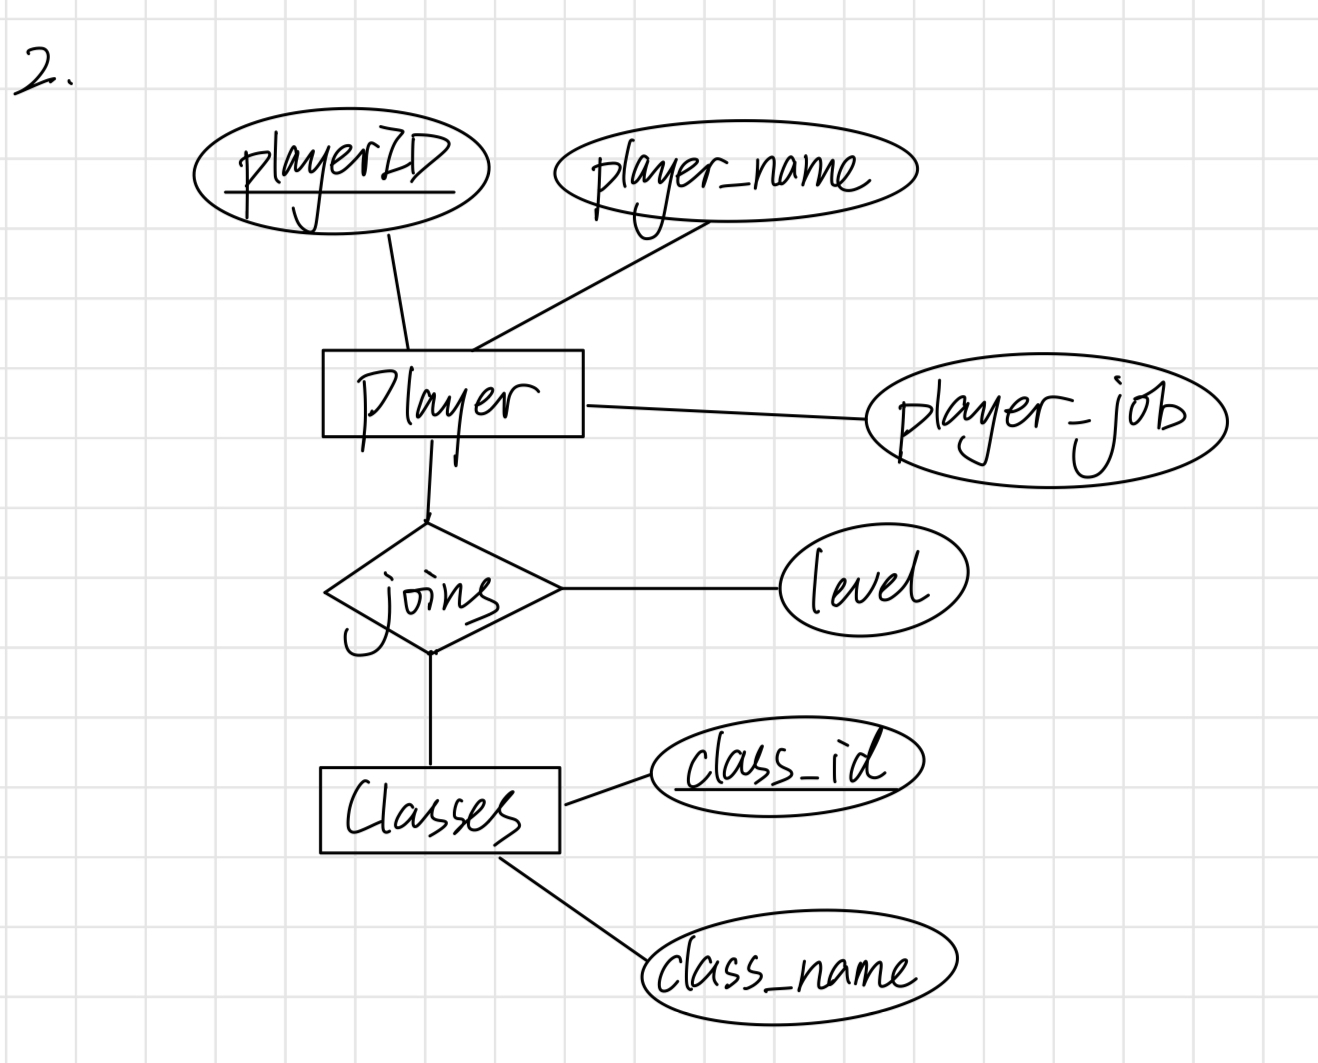
\includegraphics[width=0.5\textwidth]{p1-1-2.jpg}
\end{figure}

\newpage
\Paragraph{3.}
\begin{figure}[h]
    \centering
    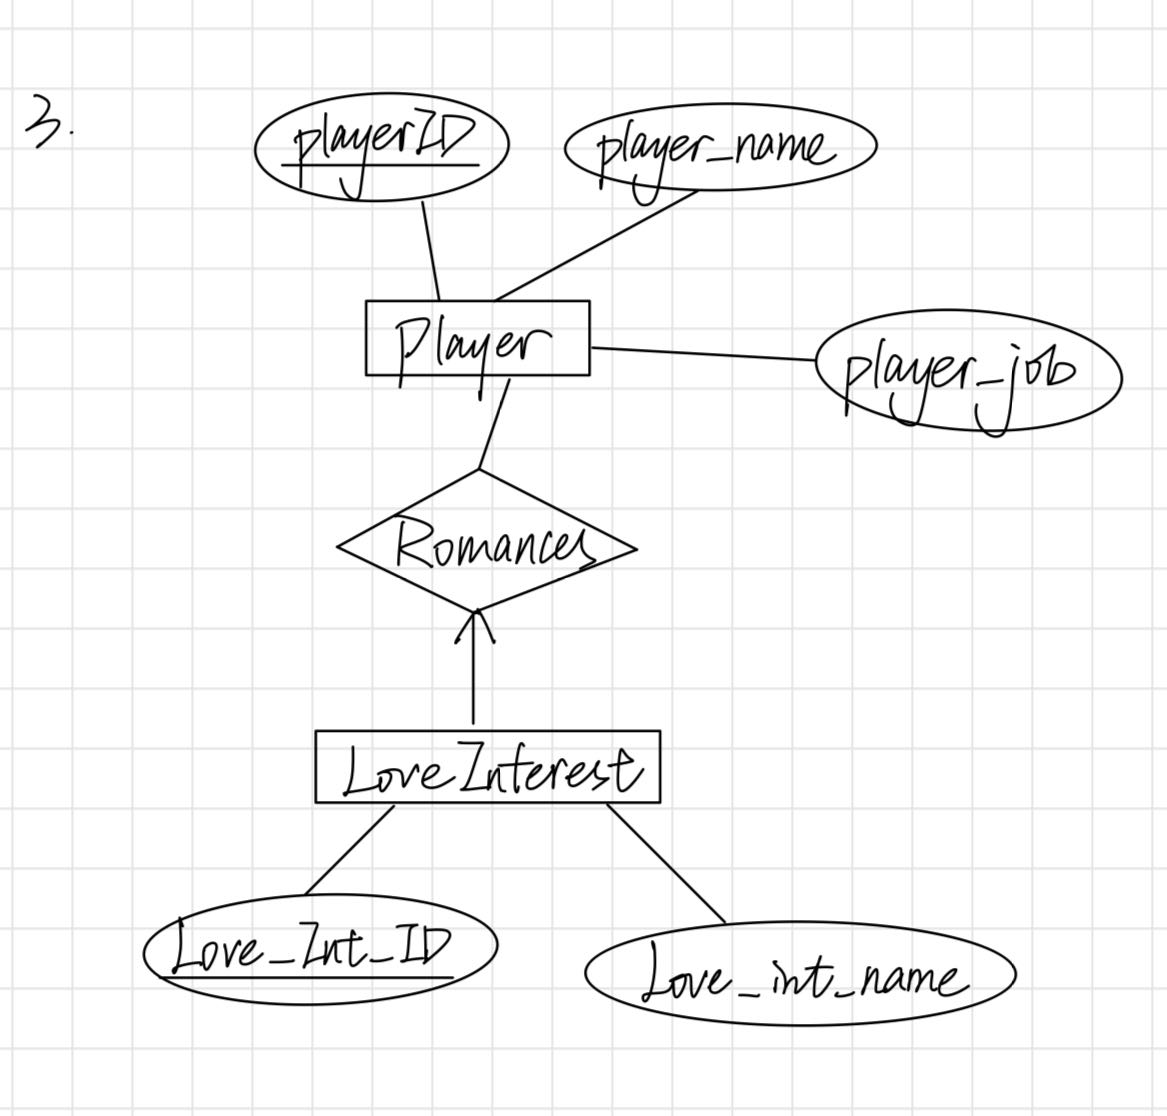
\includegraphics[width=0.6\textwidth]{p1-1-3.jpg}
\end{figure}

\Paragraph{4.}
\begin{figure}[h]
    \centering
    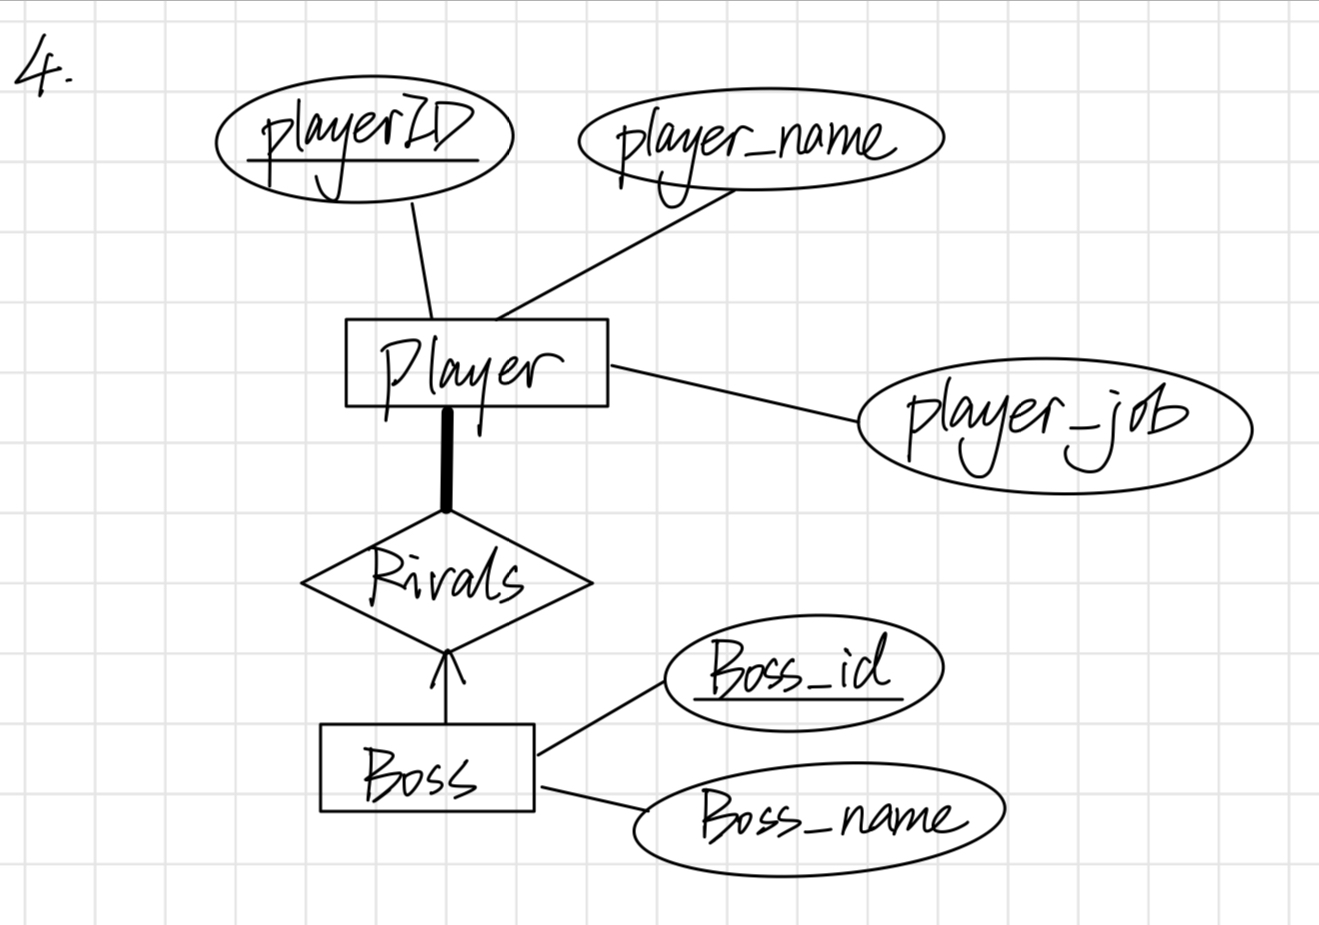
\includegraphics[width=0.6\textwidth]{p1-1-4.jpg}
\end{figure}

\newpage
\Paragraph{5.}
\begin{figure}[h]
    \centering
    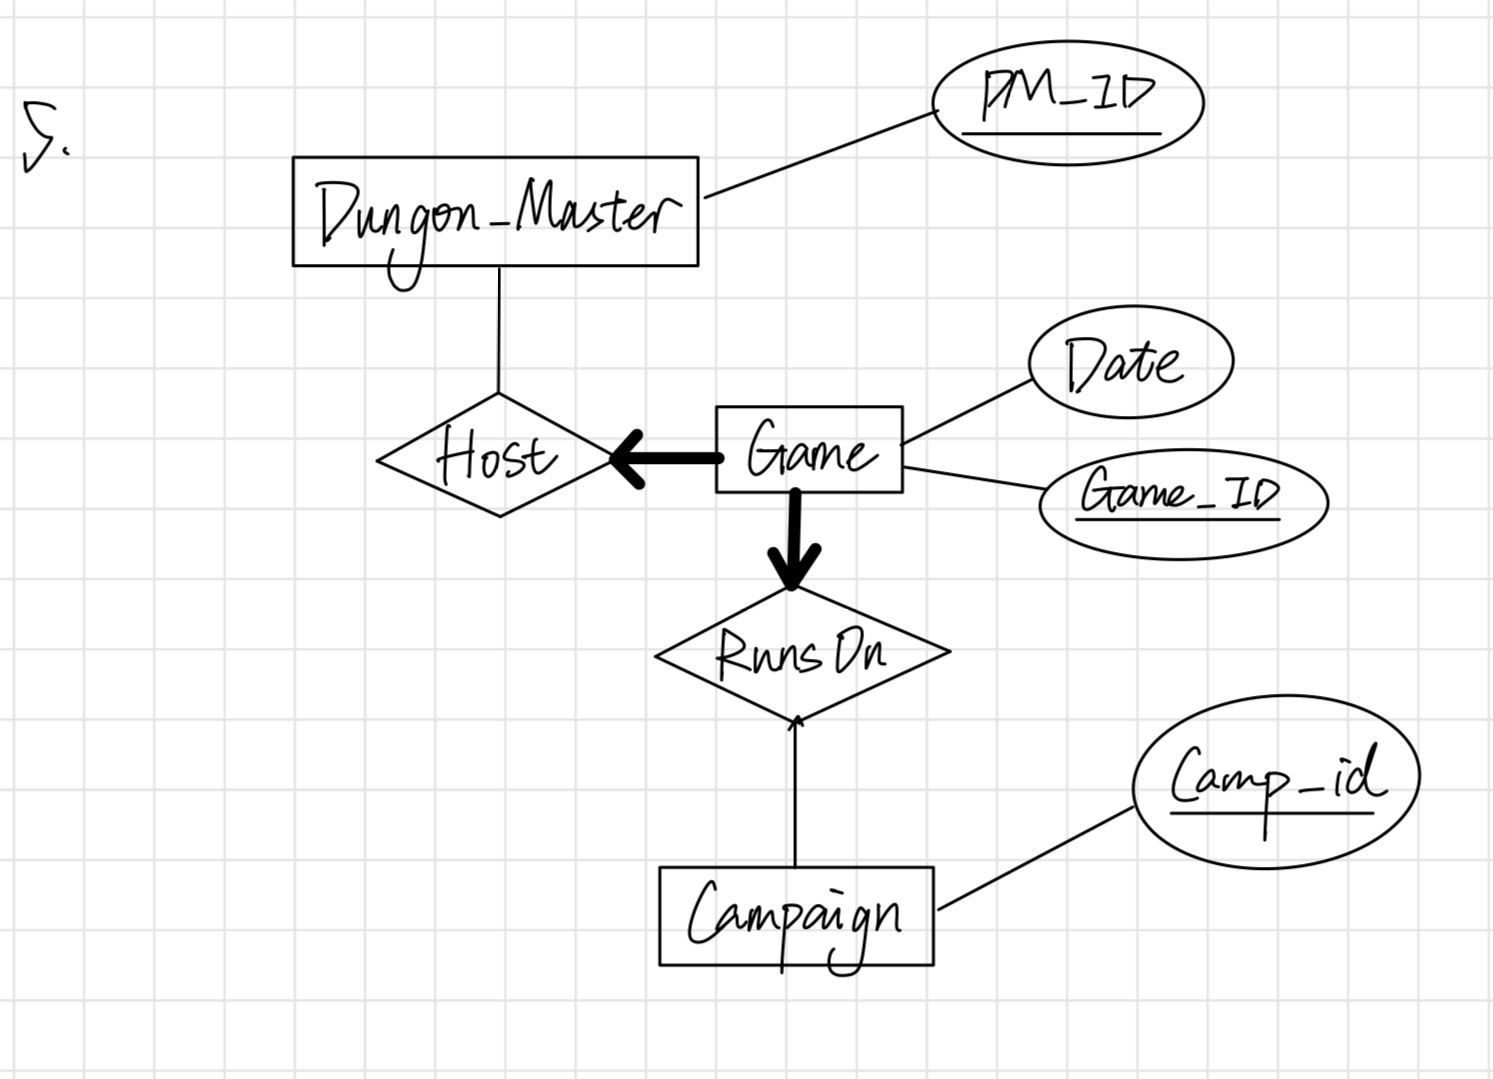
\includegraphics[width=0.6\textwidth]{p1-1-5.jpg}
\end{figure}

\Paragraph{6.}
\begin{figure}[h]
    \centering
    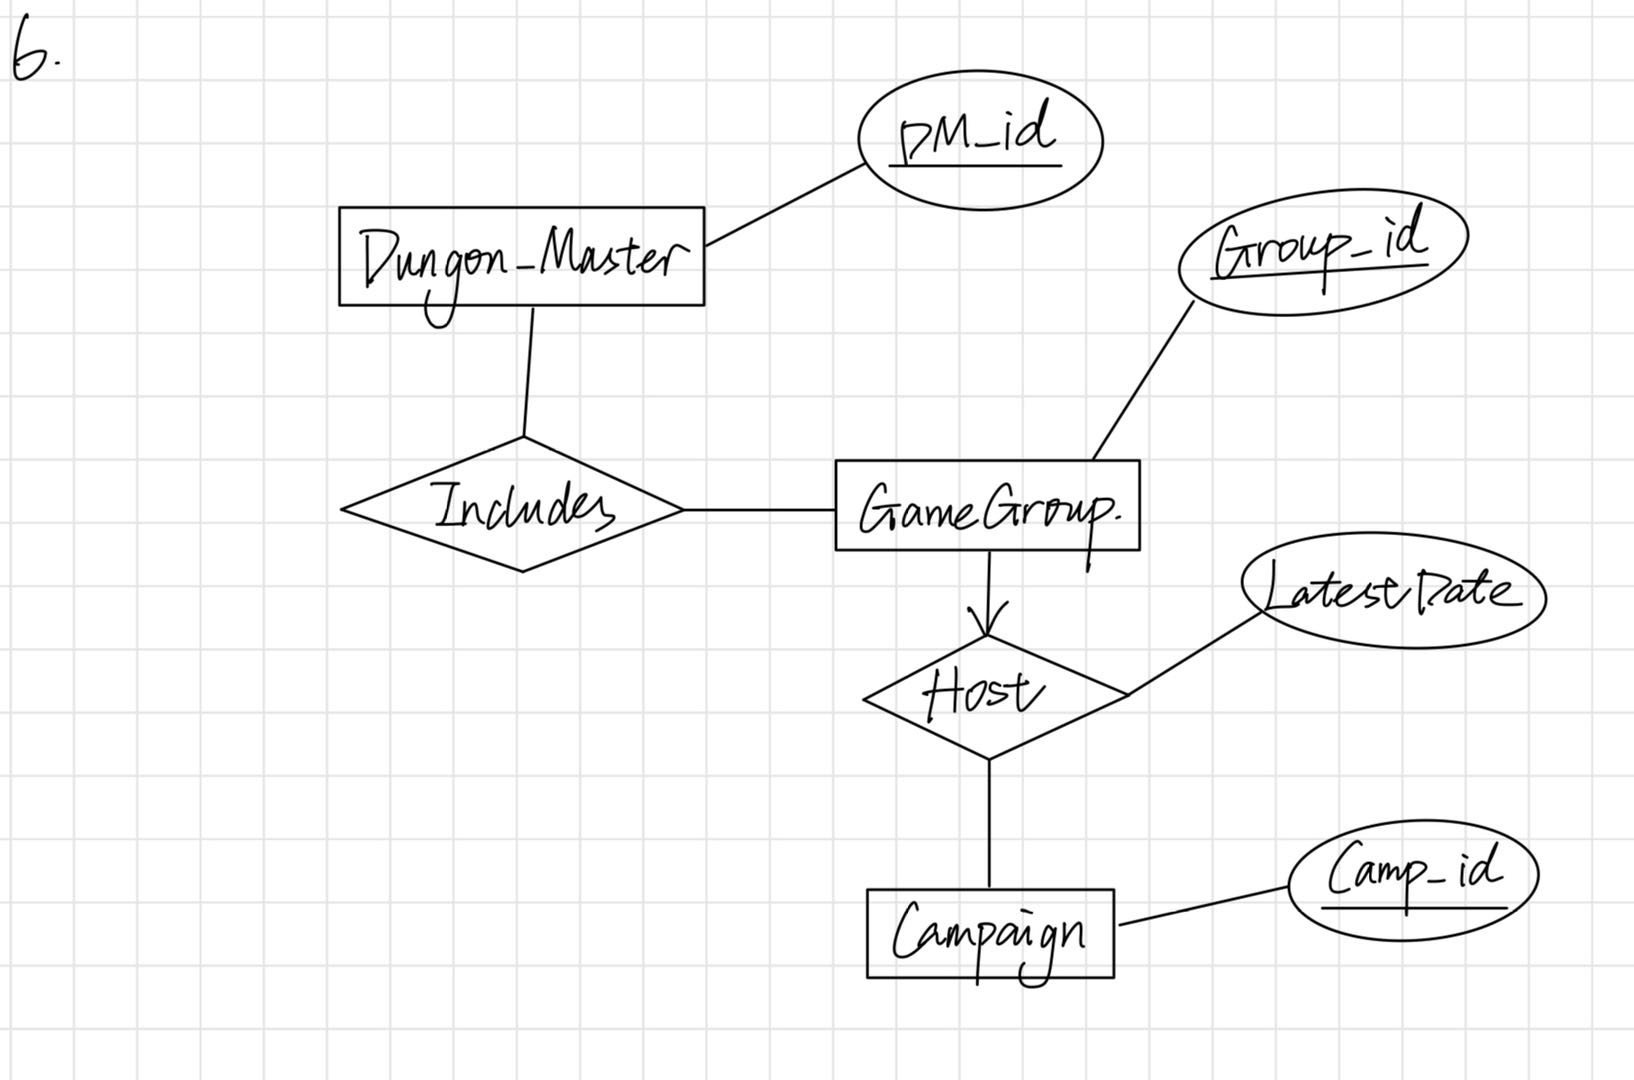
\includegraphics[width=0.6\textwidth]{p1-1-6.jpg}
\end{figure}

\newpage
\section*{Part I: Problem 2}
\Paragraph{1.}
\begin{figure}[h]
    \centering
    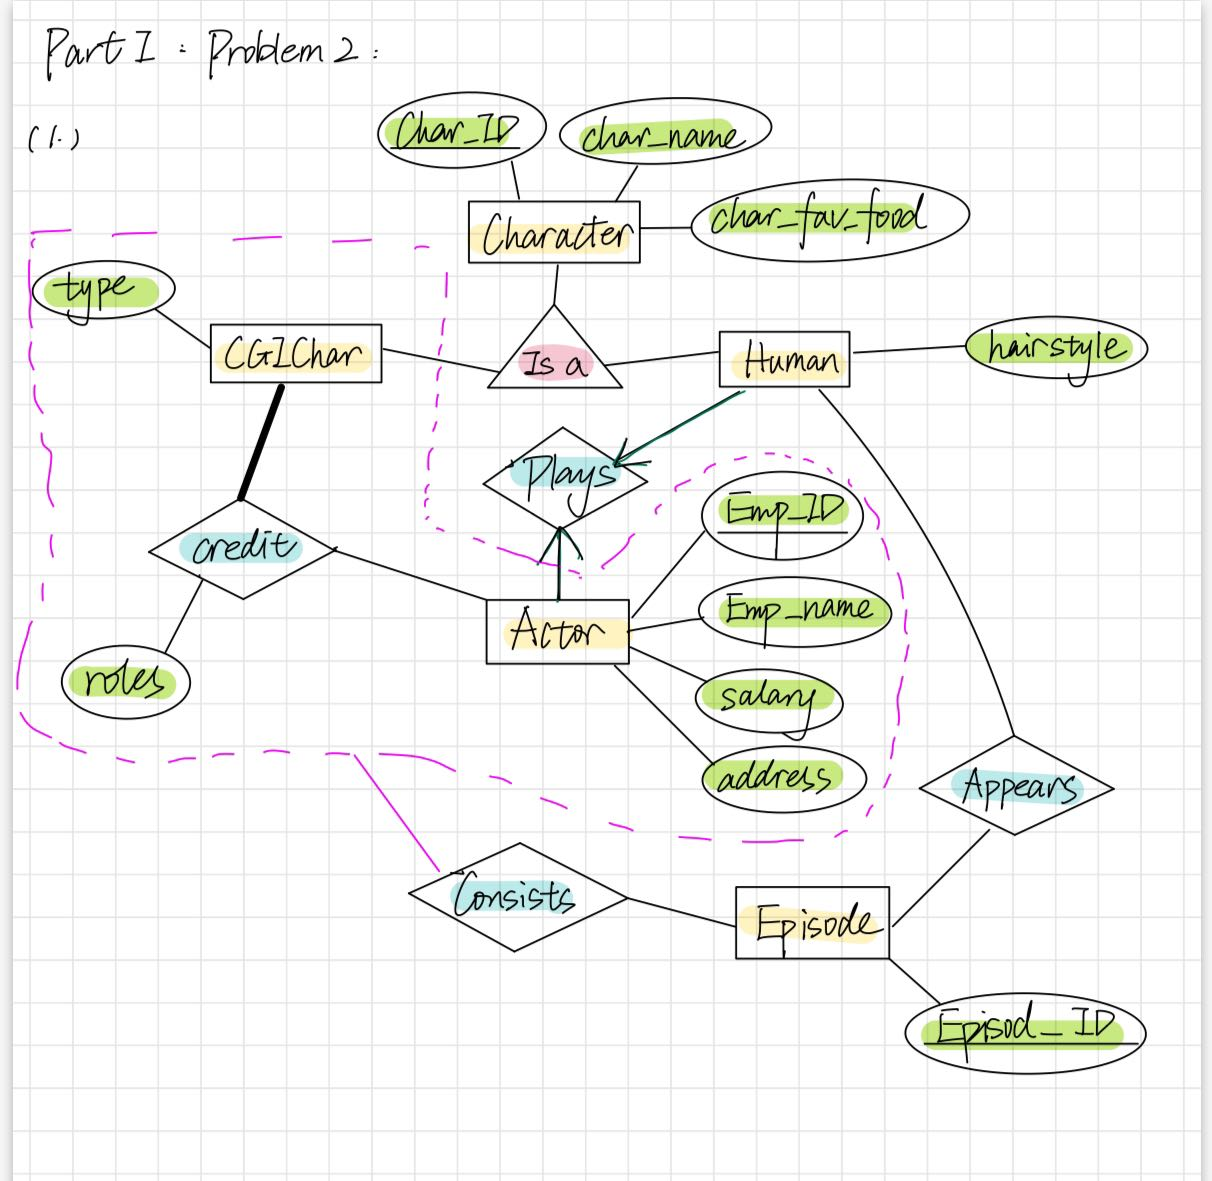
\includegraphics[width=0.8\textwidth]{p1-2-1.jpg}
\end{figure}

\newpage
\Paragraph{2.}
\begin{verbatim}
	CREATE TABLE Character (
		Char_ID INT PRIMARY KEY,
		Char_name VARCHAR(100),
		Char_fav_food VARCHAR(100)
	);

	CREATE TABLE Human (
		Char_ID INT PRIMARY KEY,
		hairstyle VARCHAR(100),
		FOREIGN KEY (Char_ID) REFERENCES Character(Char_ID)
	);

	CREATE TABLE CGIChar (
		Char_ID INT PRIMARY KEY,
		type VARCHAR(100),
		FOREIGN KEY (Char_ID) REFERENCES Character(Char_ID)
	);

	CREATE TABLE Actor (
		Emp_ID INT PRIMARY KEY,
		Emp_name VARCHAR(100),
		samealary DECIMAL(10, 2),
		address VARCHAR(100)
	);

	CREATE TABLE Plays (
		Emp_ID INT,
		Char_ID INT,
		PRIMARY KEY (Emp_ID, Char_ID),
		FOREIGN KEY (Emp_ID) REFERENCES Actor(Emp_ID),
		FOREIGN KEY (Char_ID) REFERENCES Character(Char_ID)
	);

	CREATE TABLE Credit (
		CGIChar_ID INT,
		Emp_ID INT,
		Role VARCHAR(100),
		PRIMARY KEY (CGIChar_ID, Emp_ID),
		FOREIGN KEY (CGIChar_ID) REFERENCES CGIChar(Char_ID),
		FOREIGN KEY (Emp_ID) REFERENCES Actor(Emp_ID)
	);

	CREATE TABLE Episode (
		Episode_ID INT PRIMARY KEY
	);

	CREATE TABLE Consists (
		Episode_ID INT,
		CGIChar_ID INT,
		Emp_ID INT,
		PRIMARY KEY (Episode_ID, CGIChar_ID, Emp_ID),
		FOREIGN KEY (Episode_ID) REFERENCES Episode(Episode_ID),
		FOREIGN KEY (CGIChar_ID) REFERENCES CGIChar(Char_ID),
		FOREIGN KEY (Emp_ID) REFERENCES Actor(Emp_ID)
	);

	CREATE TABLE Appears (
		Episode_ID INT, 
		HumanChar_ID INT,
		PRIMARY KEY (Episode_ID, HumanChar_ID),
		FOREIGN KEY (HumanChar_ID) REFERENCES Human(Char_ID),
		FOREIGN KEY (Episode_ID) REFERENCES Episode(Episode_ID)
	);

\end{verbatim}

\newpage
\section*{Part II: Problem 1}
\subsection*{1.}
\Paragraph{(a)\\
	For row number 1, column A, we have A = 1 \(\rightarrow\) C = 3; \\
	For row number 4, column A, we have A = 1 \(\rightarrow\) C = 4; \\
	As \(3 \neq 4\), \(A \rightarrow C\) does not hold. 
}

\Paragraph{(b)\\
	\(CD \rightarrow A\) holds, as we cannot find the exact same CD pair in the table. 
}

\Paragraph{(c)\\
	For row number 1 in column A, B and D, we have \((1, 2, 4) \rightarrow 1\) in column E; \\
	For row number 4 in column A, B and D, we have \((1, 2, 4) \rightarrow 2\) in column E; \\
	As \(1 \neq 2\), \(ABD \rightarrow E\) does not hold. 
}

\subsection*{2.}
\(A\rightarrow B\); \(A \rightarrow D\); \(A \rightarrow BD\); \\
\(D \rightarrow A\); \(D \rightarrow B\); \(D\rightarrow AB\); \\
\(E \rightarrow B\); \(E \rightarrow C\); \(E \rightarrow BC\); 

\section*{Part II: Problem 2}
\begin{figure}[h]
    \centering
    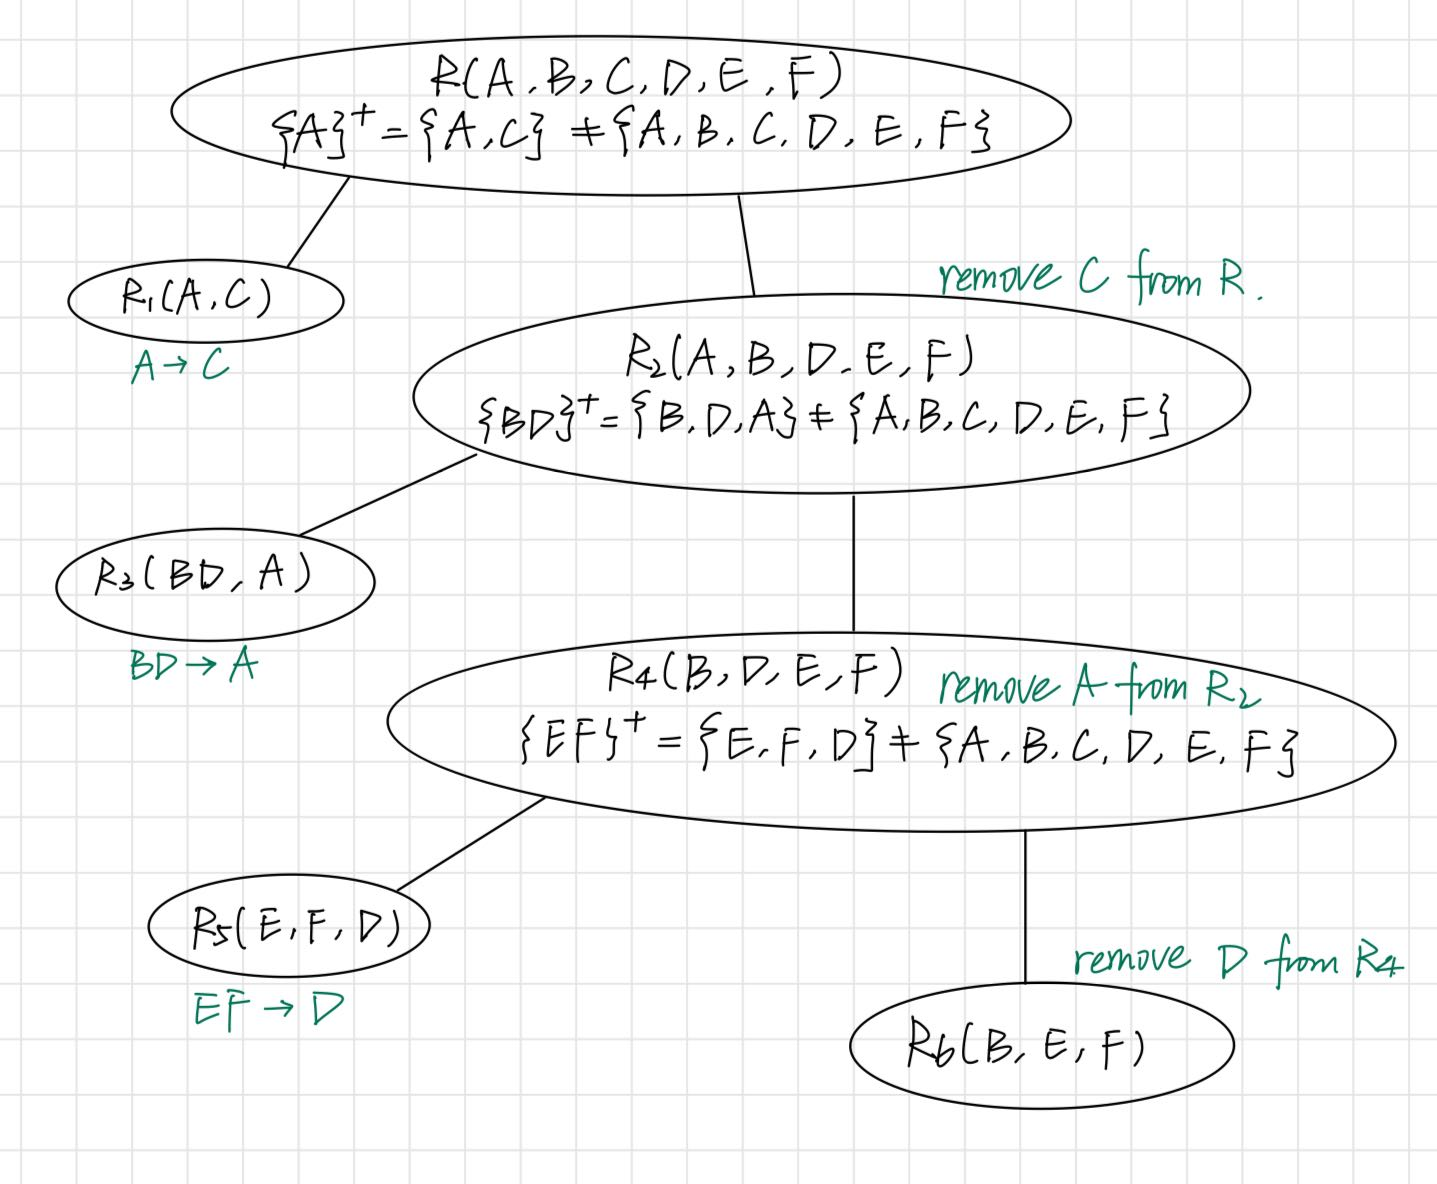
\includegraphics[width=0.6\textwidth]{p2-2.jpg}
\end{figure}
\Paragraph{
	Here is the step-by-step explaination: \\
	Step 1: Original \(R(A, B, C, D, E, F)\) and the first FD \(A \rightarrow C\). We have \(\{A\}^+ = \{A, C\} \neq \{A, B, C, D, E, F\}\).
	Then we can break down the orginal R and have \(R_1(A, C)\) and \(R_2(A, B, D, E, F)\), which removed the C as it was \(A \rightarrow C\). \\
	Step 2: From \(R_2\), we have the second FD \(BD \rightarrow C\). We will have \(\{BD\}^+ = \{B, D, A\} \neq \{A, C, B, D, E, F\}\). 
	Again, we can then break down the \(R_2\) into \(R_3(BD, A)\) and \(R_4(B, D, E, F)\), which is what we left after removing A for the same reason as C.\\
	Step 3: From  \(R_4\), we have the last FD \(EF \rightarrow D\). We have \(\{EF\}^+ = \{E, F, D\} \neq \{A, B, C, D, E, F\}\). 
	Then we break down \(R_4\) for \(EF \rightarrow D\) and have \(R_5(E, F, D)\) and \(R_6(B, E, F)\), which is what we left after we remove D for the same reason as A and C. \\
}

\section*{Part II: Problem 3}
\Paragraph{1.}
For all sets of attributes are closed, we can have "all implies empty set" as following: \\
\(A \rightarrow \emptyset\); \(B \rightarrow \emptyset\); \(C \rightarrow \emptyset\); \(D \rightarrow \emptyset\); 

\Paragraph{2.}
\(A \rightarrow BCD\); \(B \rightarrow CD\) \\
OR\\
\(A \rightarrow B\); \(B \rightarrow C\); \(C \rightarrow D\); \(D \rightarrow A\)

\Paragraph{3.}
\(A \rightarrow D\); \(B \rightarrow ACD\)\\
















\end{document}



